\documentclass[14pt, openany]{article}
\usepackage[utf8]{inputenc}
\usepackage[T1]{fontenc}
\usepackage{hyperref}
\usepackage[french]{babel}
\frenchbsetup{StandardLists=true}
\usepackage{amsmath,amsfonts,amssymb}
\usepackage{graphicx}
\usepackage[a4paper,left=2cm,right=2cm,top=2cm,bottom=2cm]{geometry}
\usepackage{bbm}
\usepackage{libertine}
\usepackage{color}
\usepackage{array,multirow,makecell}
\usepackage{enumitem} %Pour modifier les puces
\usepackage{caption}
\newcolumntype{R}[1]{>{\raggedleft\arraybackslash }b{#1}}
\newcolumntype{L}[1]{>{\raggedright\arraybackslash }b{#1}}
\newcolumntype{C}[1]{>{\centering\arraybackslash }b{#1}}
\setlength{\parindent}{0cm}
\setlength{\parskip}{1ex plus 0.5ex minus 0.2ex}
\newcommand{\hsp}{\hspace{20pt}}
\newcommand{\HRule}{\rule{\linewidth}{0.5mm}}
\AddThinSpaceBeforeFootnotes
\FrenchFootnotes

%%%% debut macro %%%%
\newenvironment{changemargin}[2]{\begin{list}{}{%
\setlength{\topsep}{0pt}%
\setlength{\leftmargin}{0pt}%
\setlength{\rightmargin}{0pt}%
\setlength{\listparindent}{\parindent}%
\setlength{\itemindent}{\parindent}%
\setlength{\parsep}{0pt plus 1pt}%
\addtolength{\leftmargin}{#1}%
\addtolength{\rightmargin}{#2}%
}\item }{\end{list}}
%%%% fin macro %%%%

\begin{document}

\begin{titlepage}
\begin{center}

\includegraphics[scale=0.15]{Images/ur2.png}\\
\bigskip
\textsc{\Large PROJET DATA SCIENCE - MASTER 2 MAS PARCOURS SCIENCES DES DONNEES\\ 
\bigskip
Rapport de l'étude}\\
\bigskip
    \HRule \\[0.4cm]
    { \huge \bfseries Prédictions des températures de 7 stations différentes à un horizon de 36 heures\\[0.4cm] }
        \HRule \\[2cm]
   \begin{figure}[h]
    \begin{minipage}[c]{.46\linewidth}
        \centering
        
\includegraphics[scale=0.3]{Images/defi.png}
    \end{minipage}
    \hfill%
    \begin{minipage}[c]{.46\linewidth}
        \centering
        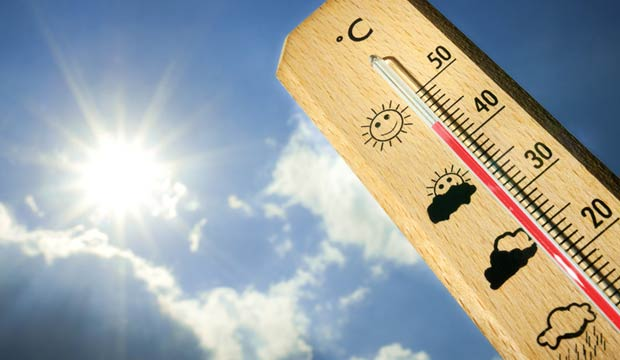
\includegraphics[scale=0.36]{Images/temp.jpg}
    \end{minipage}
	\end{figure}
    \bigskip
    \begin{minipage}{0.4\textwidth}
      \begin{flushleft} \large
      	\textsc{Benjamin ALLEAU}\\
      	\textsc{Abdessamad AZNAGUE}\\
        \textsc{Guillaume LE FLOCH}\\
        \bigskip
        Année 2017-2018\\
      \end{flushleft}
    \end{minipage}
    \begin{minipage}{0.4\textwidth}
      \begin{flushright} \large
      	\emph{Organisateur :} \textsc{INSA de Toulouse}
        \emph{Professeur encadrant :} \textsc{M. Romain TAVENARD (Université de Rennes 2)}\\
      \end{flushright}
    \end{minipage}

    \vfill
    
    % Bottom of the page
    {\large 05 Octobre 2017 —  08 Janvier 2018}

\end{center}
\end{titlepage}

\renewcommand{\contentsname}{Plan}

\tableofcontents
\newpage

\section{Présentation du projet et problématique}
\paragraph{}
La compétition 2017-2018 est basée sur une stratégie d'adaptation statistique pour améliorer la prévision de températures à un horizon de 36 heures.

Les services du \textbf{CNRM} (Centre National de Recherches Météorologiques) construisent des grands modèles déterministes de l'atmosphère par résolution des équations de Navier et Stockes sur un maillage: 10km pour \textbf{ARPEGE}, kilométrique pour \textbf{AROME} mais limité à l'Europe. Il apparaît que ces modèles sont généralement biaisés, notamment parce qu'ils ne peuvent prendre en compte des phénomènes à petite échelle. Par exemple, un vent important (e.g. vent d'autan à Toulouse) provoque des turbulences qui, en mélangeant les couches d'air, entrainent une baisse de la température par rapport à celle prévue.

Un modèle statistique intégrant les prévisions du modèle déterministe peut contribuer à réduire significativement ces biais. En revanche, un modèle statistique seul est incapable de prévoir l'arrivée d'une perturbation océanique à partir de données locales. L'adaptation statistique est donc une mise en collaboration \og optimale \fg{} des deux approches de modélisation, déterministe et statistique.

Le \og Défi Grosses Data \fg{} est donc un challenge mettant en confrontation une multitude de groupes d'étudiants provenant des \textbf{INSA} de Toulouse et Rennes, ainsi que des Universités de \textbf{Bordeaux}, \textbf{Rennes 1}, \textbf{Rennes 2}, \textbf{Paris Descartes}, \textbf{Paul Sabatier (Toulouse 3)} ou encore la \textbf{Toulouse School of Economics}. Ce rapport détaillera le travail fourni par l'équipe \textbf{Freak-unit}, une des 8 équipes représentant l'\textbf{Université de Rennes 2}.

L'objectif de ce projet est simple : prédire au mieux les températures de 7 stations sur un horizon de 36 heures. Pour ce faire, 36 fichiers $train\_H.csv$, $H=1,..,n$, ont été mis à notre disposition. Ces fichiers contiennent les variables issues des modèles physiques décrits dans le préambule à un horizon de +H heures. Leur contenu est le suivant :
\begin{itemize}
\item les lignes correspondent à chaque jour sur une période allant du $1^{er}$ janvier 2014 au 30 mai 2016.
\item les colonnes contiennent 30 variables (température, nébulosité, vent, humidité ..)
\end{itemize}
Nous allons détailler ces variables afin de bien comprendre quelles sont les mesures à notre disposition :
\begin{itemize}
\item \textbf{insee} : Facteur à 7 niveaux représentant le numéro insee des stations pour lesquelles nous cherchons à prédire les températures (Nice, Toulouse Blagnac, Bordeaux-Mérignac, Rennes, Lille Lesquin, Strasbourg Entzheim, Paris-Montsouris)
\item \textbf{tH2\_obs} : Observation de la température à 2 mètres \textit{in situ} au point station (prédictant). \textbf{C'est la variable réponse que l'on cherche à prédire}
\item \textbf{ech} : Facteur à 36 niveaux correspondant à l'échéance de validité (H)
\item \textbf{capeinsSOL0} : Energie potentielle convective
\item \textbf{ciwcH20} : Fraction de glace nuageuse à 20 mètres
\item \textbf{clwcH20} : Fraction d'eau nuageuse à 20 mètres
\item \textbf{nH20} : Fraction nuageuse à 20 mètres
\item \textbf{pMER0} : Pression au niveau de la mer
\item \textbf{rr1SOL0} : Précipitation horaire au niveau du sol
\item \textbf{rrH20} : Précipitation horaire à 20 mètres
\item \textbf{tpwHPA850} : Température potentielle au niveau 850 hPa
\item \textbf{ux1H10} : Rafale 1 minute du vent à 10 mètres composante zonale
\item \textbf{vapcSOL0} : Colonne de vapeur d'eau
\item \textbf{vx1H10} : Rafale 1 minute du vent à 10 mètres composante verticale
\item \textbf{ddH10\_rose4} : Facteur à 4 niveaux indiquant la direction du vent à 10 mètres (en rose4)
\item \textbf{ffH10} : Force du vent à 10 mètres en m/s
\item \textbf{flir1SOL0} : Flux Infra-rouge en J/$m^2$
\item \textbf{fllat1SOL0} : Flux de chaleur latente en J/$m^2$
\item \textbf{flsen1SOL0} : Flux de chaleur sensible en J/$m^2$
\item \textbf{flvis1SOL0} : Flux visible en J/$m^2$
\item \textbf{hcoulimSOL0} : Hauteur de la couche limite en mètres
\item \textbf{huH2} : Humidité 2mètres en \%
\item \textbf{iwcSOL0} : Réservoir neige kg/$m^2$ (équivalent en eau liquide des chutes de neige
\item \textbf{nbSOL0\_HMoy} : Nébulosité basse (moyenne sur les 6 points de grille autour de la station) (fraction en octat du ciel occulté)
\item \textbf{ntSOL0\_HMoy} : Nébulosité totale (moyenne sur les 6 points de grille autour de la station)
\item \textbf{tH2} : Température à 2 mètres du modèle \textbf{AROME}
\item \textbf{tH2\_VGrad\_2.100} : Gradient vertical de température entre 2 mètres et 100 mètres
\item \textbf{tH2\_XGrad} : Gradient zonal de température à 2 mètres
\item \textbf{tH2\_YGrad} : Gradient méridien de température à 2 mètres
\item \textbf{mois} : Facteur à 12 niveaux représentant le mois
\end{itemize}
Il est à noter que ces 36 fichiers \textit{train} contiennent des valeurs manquantes, le sujet sera approfondi un peu plus tard dans l'étude.

L'objectif de ce projet est le suivant : à partir des différents fichiers \textit{train} nous devons réaliser un apprentissage (supervisé dans notre cas) afin de pouvoir appliquer par la suite notre modèle au fichier \textit{test.csv} qui contient les mêmes variables, à l'exception de \textbf{tH2\_obs} évidemment puisqu'il faut la prédire. Les lignes du fichier \textit{test.csv} contiennent les 6 périodes de 15 jours suivantes :
\begin{itemize}
\item du 20/06/2016 au 02/07/2016
\item du 01/08/2016 au 14/08/2016
\item du 12/09/2016 au 25/09/2016
\item du 24/10/2016 au 06/11/2016
\item du 05/12/2016 au 18/12/2016
\item du 08/05/2017 au 21/05/2017
\end{itemize}
Une fois les prédictions effectuées, il faut soumettre les résultats sous forme d'un fichier au format \textit{csv} toujours, sur le site internet du challenge. Au bout d'exactement 1 heure après la soumission, nous pouvons visualiser notre score. La métrique utilisée pour évaluer le score est le \textbf{RMSE} (Root Mean Square Error). Si l'on note $\hat{y}$ notre vecteur de prédictions et $y_{obs}$ les valeurs des températures réellement observées, le \textbf{RMSE} associé se note :\\
\begin{center}
$RMSE_{\hat{y}} = \sqrt{\frac{1}{n} \sum\limits_{i=1}^n (\hat{y_i}-y_{obs_i})^2}$
\end{center}
En d'autres termes, cette métrique permet de mesurer d'une certaine façon l'écart entre nos prédictions et la réalité. Il est à noter que le challenge fournit un score de $1.30755$ appelé \textbf{Baseline} qui correspond à un score de référence, associé à \og un modèle élémentaire de prévision sans effort particulier d'optimisation. C'est un objectif a minima à améliorer dans ce concours \fg{}. Le décor est planté, désormais il ne reste plus qu'à se lancer dans le challenge.
\section{Remerciements}
\paragraph{}
Avant de détailler les différentes étapes de ce projet, les 3 membres de la \textbf{Freak-Unit} team souhaitent remercier tout particulièrement leur professeur encadrant, \textbf{M. Romain TAVENARD} pour son accompagnement tout au long du projet et pour l'aide apportée. Sa connaissance du \textit{Deep Learning} notamment, aura été un facteur déterminant dans la réussite de ce projet.

\section{Les différentes étapes du projet}

\subsection{Différentes stratégies envisagées}

\subsection{Analyse des corrélations entre variables et visualisation}

\subsection{Gestion et remplacement des valeurs manquantes}

\subsection{Choix et application d'algorithmes d'apprentissage supervisé}

\subsubsection{Premiers algorithmes : la régression linéaire et ses variantes}

\subsubsection{Forêt aléatoire : l'algorithme Random Forest}

\subsubsection{Gradient Boosting : l'algorithme XGBoost}

\subsubsection{Deep Learning : l'utilisation des réseaux de neurones}

\section{Bilan}

\section{Bibliographie}

\end{document}